\documentclass[11pt]{article}

% NOTE: For NeurIPS submission, replace this preamble with:
%   \usepackage[preprint]{neurips_2025}
% and remove the geometry package.

\usepackage[utf8]{inputenc}
\usepackage[T1]{fontenc}
\usepackage{amsmath,amssymb,amsthm}
\usepackage{mathtools}
\usepackage{hyperref}
\usepackage{cleveref}
\usepackage{booktabs}
\usepackage{enumitem}
\usepackage[margin=1in]{geometry}
\usepackage{xcolor}
\usepackage{tikz}
\usetikzlibrary{patterns,decorations.pathreplacing,calc}

\newtheorem{theorem}{Theorem}[section]
\newtheorem{lemma}[theorem]{Lemma}
\newtheorem{corollary}[theorem]{Corollary}
\newtheorem{proposition}[theorem]{Proposition}
\newtheorem{definition}[theorem]{Definition}
\newtheorem{remark}[theorem]{Remark}
\newtheorem{example}[theorem]{Example}
\newtheorem{counterexample}[theorem]{Counterexample}

\newcommand{\R}{\mathbb{R}}
\newcommand{\N}{\mathbb{N}}
\newcommand{\cl}[1]{\overline{#1}}
\newcommand{\Fix}{\operatorname{Fix}}
\newcommand{\AD}{\operatorname{AD}}
\newcommand{\id}{\operatorname{id}}
\newcommand{\diam}{\operatorname{diam}}
\newcommand{\dist}{\operatorname{dist}}

\title{The Defense Trilemma:\\
  Impossibility of Continuous Utility-Preserving Wrapper Defenses}

\author{
    {\rm Manish Bhatt\thanks{Corresponding author: manish.bhatt13212@gmail.com}}\hspace{0.5em}\footnotemark[2]\\
    OWASP
    \and
    {\rm Sarthak Munshi}\footnotemark[2]\\
    Amazon Web Services
  \and
  {\rm Vineeth Sai Narajala}\footnotemark[2]\\
  Cisco
  \and
  {\rm Idan Habler}\footnotemark[2]\\
  Cisco
  \and
  {\rm Ammar Al-Kahfah}\footnotemark[2]\\
  Amazon Web Services
  \and
  {\rm Ken Huang}\\
  Distributedapps.ai
  \and
  {\rm Blake Gatto}\\
  Shrewd Security
  }

\date{}

\begin{document}

\maketitle
\renewcommand{\thefootnote}{\fnsymbol{footnote}}
 \footnotetext[2]{Equal contribution. This work was conducted independently and does not reflect the views, policies, or endorsements of the
  authors' respective employers.}
 \footnotetext[3]{This work was conducted independently and does not reflect the views, policies, or endorsements of the
  authors' respective employers.}
\begin{abstract}
We prove that no continuous, utility-preserving wrapper defense 
function $D\colon X\to X$ that preprocesses inputs before the model
sees them, can eliminate all safety violations from a language model
with connected prompt space, and we characterize exactly where every
such defense must fail. We establish three results of increasing
strength: \emph{boundary fixation}---the defense must leave some
threshold-level inputs unchanged; an \emph{$\varepsilon$-robust
constraint}---under Lipschitz regularity, a positive-measure band
around fixed boundary points remains near-threshold; and a
\emph{persistent unsafe region}---under a transversality condition, a
positive-measure subset of inputs remains strictly unsafe. These
constitute a \emph{defense trilemma}: continuity, utility preservation,
and completeness cannot coexist. We prove parallel discrete results
requiring no topology, and extend to multi-turn interactions,
stochastic defenses, and capacity-parity settings. The results do not
preclude training-time alignment, architectural changes, or defenses
that sacrifice utility. The full theory is mechanically verified in
Lean~4 with Mathlib
\url{https://github.com/mbhatt1/stuff/tree/main/ManifoldProofs}
(45 files, ${\sim}350$ theorems, no admitted proofs, three standard
axioms) and validated empirically on three LLMs~\cite{munshi2026manifold}.
\end{abstract}


% ============================================================
\section{Introduction}
\label{sec:intro}

Can you build a wrapper around a language model that eliminates all
prompt injection vulnerabilities? Most current defense work implicitly
assumes yes. Input classifiers that flag suspicious
prompts~\cite{alon2023detecting}, output filters that catch unsafe
completions~\cite{inan2023llama}, and constitutional rewriting
pipelines~\cite{bai2022constitutional} all share the same structure: a
function $D\colon X \to X$ that preprocesses prompts before the model
sees them, mapping unsafe inputs to safe equivalents while leaving safe
inputs unchanged. We prove the answer is no, under two mild constraints. If the defense
is \emph{continuous} (similar prompts produce similar rewrites) and
\emph{utility-preserving} (safe prompts pass through unchanged), it
cannot be \emph{complete} (make every output safe). These three
properties form a \textbf{defense trilemma}: any two can coexist, but
not all three (\Cref{fig:trilemma}).

The impossibility is not about specific attacks or clever prompt
engineering. It arises from the \emph{geometry} of the prompt space
itself: in a connected space, the safe region is open but not closed,
so any continuous defense that fixes safe inputs must also fix points
on the safety boundary. We establish three results, each strictly
stronger than the last (\Cref{fig:escalation} provides visual
intuition):

\paragraph{Boundary fixation (\Cref{thm:main}).}
The defense must fix at least one boundary point, i.e., a prompt where
alignment deviation equals the threshold exactly---passing it through
with no remediation.

\paragraph{$\varepsilon$-robust constraint (\Cref{thm:eps-robust}).}
Under Lipschitz regularity, the defense cannot uniformly reduce
alignment deviation far below~$\tau$ near the fixed boundary point.
For any $x$ within distance $\delta$ of the fixed point~$z$:
\begin{equation}\label{eq:eps-bound}
  f(D(x)) \;\geq\; \tau - L(K+1)\,\delta.
\end{equation}

\paragraph{Persistent unsafe region (\Cref{thm:persistent}).}
Under a transversality condition, the alignment surface rises faster
than the defense can pull it down, leaving a positive-measure region
that remains unsafe:
\begin{equation}\label{eq:persistent}
  f(D(x)) > \tau \quad\text{for all } x \in \mathcal{S},
  \qquad \mu(\mathcal{S}) > 0.
\end{equation}

\paragraph{From discrete to continuous.}
All three results apply to continuous interpolants of discrete data.
The Tietze extension theorem guarantees that any finite set of
behavioral observations in a normal space admits continuous extensions,
and the impossibilities hold for every such extension
(\Cref{thm:tietze}).

\medskip
\noindent\textbf{Scope and limitations.}
Our results apply specifically to \emph{continuous, utility-preserving
wrapper defenses} on \emph{connected} prompt spaces. They do \emph{not}
preclude effective safety through other mechanisms, including:
\begin{itemize}[nosep]
  \item training-time alignment (RLHF, DPO, constitutional AI training),
  \item architectural changes to the model itself,
  \item discontinuous defenses (e.g., hard blocklists or discrete classifiers),
  \item multi-component systems whose classifiers may reject or redirect
        inputs rather than preserving utility on every prompt.
\end{itemize}

All three conditions---continuity, utility preservation, and
connectedness, are individually necessary; we give counterexamples for
each (\Cref{app:counterexamples}). The core theory and all extensions
are mechanically verified in Lean~4 with zero \texttt{sorry} statements.
Full proofs appear in \Cref{app:proofs}; the Lean artifact is described
in \Cref{app:artifact}.


% ============================================================
\section{Related Work}
\label{sec:related}

Adversarial robustness research has established that small
perturbations can fool classifiers~\cite{szegedy2013intriguing,
goodfellow2014explaining,carlini2017evaluating,madry2018towards} and
that robustness may fundamentally trade off against
accuracy~\cite{tsipras2018robustness,fawzi2018adversarial}. Certified
defenses provide guarantees for fixed
models~\cite{cohen2019certified,katz2017reluplex,singh2019abstract,
huang2017safety,bagnall2019certifying}, and topological perspectives
have illuminated the structure of decision
boundaries~\cite{naitzat2020topology}. For LLMs specifically,
jailbreaking attacks~\cite{zou2023universal,chao2024jailbreaking,
mehrotra2024tree,greshake2023indirect} and automated
red-teaming~\cite{mouret2015illuminating,samvelyan2024rainbow}
demonstrate persistent vulnerabilities.

Our work differs in kind: rather than studying how failures arise for
fixed models or how specific systems can be certified, we impose
\emph{universal constraints on the defense map itself}. The closest
conceptual precedent is the no-free-lunch
framework~\cite{wolpert1997no}, which proves that no optimizer
dominates across all problems. We prove the analogous result for
wrapper defenses: under continuity and utility preservation, no
defense eliminates all failures.


% ============================================================
\section{Formal Framework}
\label{sec:setup}

Before defining the model formally, we sketch the intuition. Every
prompt lives in a space~$X$. A scoring function~$f$ assigns each prompt
a number measuring how far the model's response deviates from alignment
goals: low scores are safe, high scores are unsafe. A fixed
threshold~$\tau$ separates the two. A \emph{defense} preprocesses
prompts before the model sees them, trying to push unsafe prompts into
safe territory. We require two natural properties: \emph{continuity}
(similar prompts produce similar rewrites, i.e., no brittle edge-case
behavior) and \emph{utility preservation} (safe prompts pass through
unchanged, so the defense does not degrade normal use).
\Cref{fig:landscape} illustrates the setup.

\begin{figure}[t]
\centering
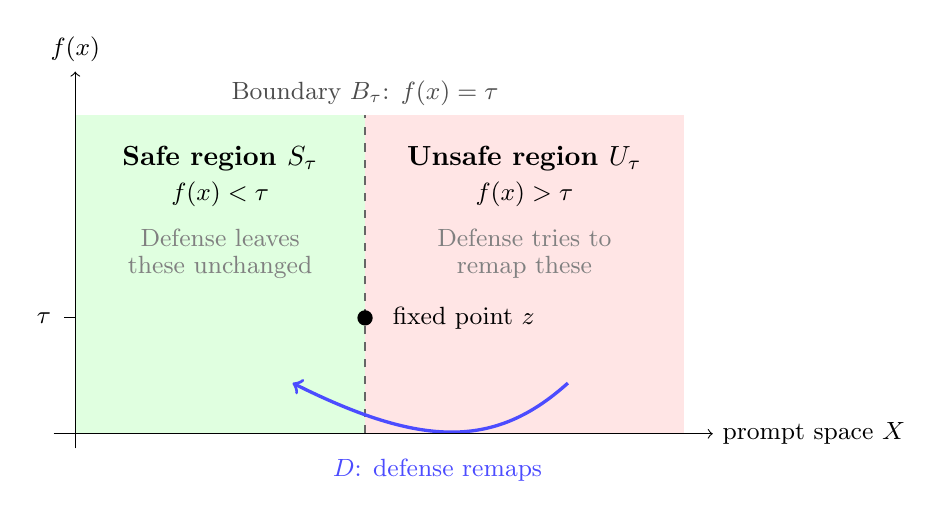
\begin{tikzpicture}[scale=0.92]
  \fill[green!12] (0,0.8) rectangle (4.0,5.2);
  \fill[red!10] (4.0,0.8) rectangle (8.4,5.2);
  \draw[dashed, thick, black!60] (4.0,0.8) -- (4.0,5.2);
  \node[font=\bfseries] at (2.0,4.6) {Safe region $S_\tau$};
  \node[font=\small] at (2.0,4.1) {$f(x) < \tau$};
  \node[font=\small, black!50] at (2.0,3.5) {Defense leaves};
  \node[font=\small, black!50] at (2.0,3.1) {these unchanged};
  \node[font=\bfseries] at (6.2,4.6) {Unsafe region $U_\tau$};
  \node[font=\small] at (6.2,4.1) {$f(x) > \tau$};
  \node[font=\small, black!50] at (6.2,3.5) {Defense tries to};
  \node[font=\small, black!50] at (6.2,3.1) {remap these};
  \node[font=\small, black!70] at (4.0,5.5) {Boundary $B_\tau$: $f(x)=\tau$};
  \fill[black] (4.0,2.4) circle (3pt);
  \node[anchor=west, font=\small] at (4.25,2.4) {fixed point $z$};
  \draw[->, thick, blue!70, line width=1.2pt]
    (6.8,1.5) .. controls (5.8,0.6) and (4.8,0.6) .. (3.0,1.5);
  \node[font=\small, blue!70] at (5.0,0.3) {$D$: defense remaps};
  \draw[->] (-0.3,0.8) -- (8.8,0.8) node[right] {\small prompt space $X$};
  \draw[->] (0,0.6) -- (0,5.8) node[above] {\small $f(x)$};
  \draw (0,2.4) -- (-0.15,2.4);
  \node[anchor=east, font=\small] at (-0.2,2.4) {$\tau$};
\end{tikzpicture}
\caption{Schematic of the prompt space. The defense~$D$ must leave all
safe inputs unchanged (utility preservation) and tries to remap unsafe
inputs into the safe region. Boundary fixation (\Cref{thm:main}) proves
the defense must also leave some boundary points unchanged, the black
dot~$z$ passes through with no remediation.}
\label{fig:landscape}
\end{figure}

\begin{definition}[Alignment Deviation Function]
\label{def:ad}
Let $X$ be a topological space (a set equipped with a notion of
``nearness'' between points). An \emph{alignment deviation function} is
a continuous map $f\colon X \to \R$, i.e., small changes in the
input produce small changes in the score. Given a threshold
$\tau\in\R$:
\begin{align}
  S_\tau &= \{x \in X : f(x) < \tau\}  &&\text{(safe region)} \\
  U_\tau &= \{x \in X : f(x) > \tau\}  &&\text{(unsafe region)} \\
  B_\tau &= \{x \in X : f(x) = \tau\}  &&\text{(boundary)}
\end{align}
\end{definition}

\begin{definition}[Defense]
\label{def:defense}
A \emph{defense} is a continuous map $D\colon X \to X$. It is
\emph{utility-preserving} if $D(x) = x$ for all $x \in S_\tau$
(safe prompts pass through unchanged),
and \emph{complete} if $f(D(x)) < \tau$ for all $x\in X$
(every output is safe).
\end{definition}

\begin{example}[Running example]
\label{ex:running}
Consider $X = [0,1]$, $f(x) = x$, $\tau = 0.5$. The safe region is
$[0, 0.5)$, the unsafe region is $(0.5, 1]$, and the boundary is
$\{0.5\}$. A utility-preserving defense must satisfy $D(x) = x$ for all
$x < 0.5$. Continuity then forces $D(0.5) = \lim_{x \to 0.5^-} D(x)
= 0.5$, so the boundary point is fixed: $f(D(0.5)) = 0.5 = \tau$. No
matter how cleverly the defense handles inputs above~$0.5$, the point
$x = 0.5$ slips through. We will see that this simple observation
generalizes to arbitrary connected spaces and grows sharper under
regularity assumptions.
\end{example}

The central question is whether a defense can be both
utility-preserving and complete. The following sections show that under
natural conditions the answer is no.


% ============================================================
\section{Boundary Fixation}
\label{sec:boundary}

We begin with the most fundamental result. The argument fits in a
paragraph: the defense fixes every safe input, so continuity makes its
fixed-point set closed. But the safe region~$S_\tau$ is open (preimage
of an open interval under continuous~$f$), and in a connected space a
nonempty proper open set is not closed. Hence the fixed-point set
cannot stop exactly at the edge of the safe region, it must spill onto
the boundary~$B_\tau$. Some boundary prompts pass through unchanged.

\begin{theorem}[Boundary Fixation]
\label{thm:main}
Let $X$ be a connected Hausdorff space (a space that is ``in one
piece'' and where distinct points can be separated by neighborhoods).
Let $f\colon X\to\R$ be continuous with $S_\tau, U_\tau \neq
\emptyset$, and $D\colon X \to X$ continuous with
$D|_{S_\tau} = \id$. Then there exists $z\in X$ with $f(z) = \tau$
and $D(z) = z$. Moreover, every $z \in \cl{S_\tau} \setminus S_\tau$
satisfies $f(z) = \tau$ and $D(z) = z$, and this set is nonempty.
\end{theorem}

\begin{proof}[Proof sketch]
In a Hausdorff space, $\Fix(D)$ is closed (preimage of the diagonal).
By utility preservation, $S_\tau \subseteq \Fix(D)$, so
$\cl{S_\tau} \subseteq \Fix(D)$. But $S_\tau = f^{-1}((-\infty,\tau))$
is open and not closed (connectedness: a nonempty proper clopen set
would disconnect~$X$). Hence $\cl{S_\tau} \supsetneq S_\tau$. Any
$z \in \cl{S_\tau}\setminus S_\tau$ satisfies $f(z) = \tau$ (limits of
values ${<}\tau$ cannot exceed~$\tau$, and $z \notin S_\tau$ forces
$f(z) \geq \tau$) and $D(z) = z$. Full proof in \Cref{app:proofs}.
\end{proof}

The defense's fixed-point set is too large to avoid the
boundary. Utility preservation forces it to contain the safe region;
closure forces it to contain the boundary; connectedness ensures the
boundary is nonempty. Equivalently: a complete utility-preserving
defense would be a continuous retraction $D\colon X \to S_\tau$
(since $D|_{S_\tau} = \id$ and $D(X) \subseteq S_\tau$), but a
retract of a connected space is closed, while~$S_\tau$ is open and
proper---a contradiction.

\begin{corollary}
No continuous utility-preserving defense is complete.
\end{corollary}

All three hypotheses are individually necessary. A defense can satisfy
at most two of the three---the \emph{defense trilemma}
(\Cref{fig:trilemma}). Counterexamples for each dropped hypothesis
appear in \Cref{app:counterexamples}.

\begin{figure}[t]
\centering
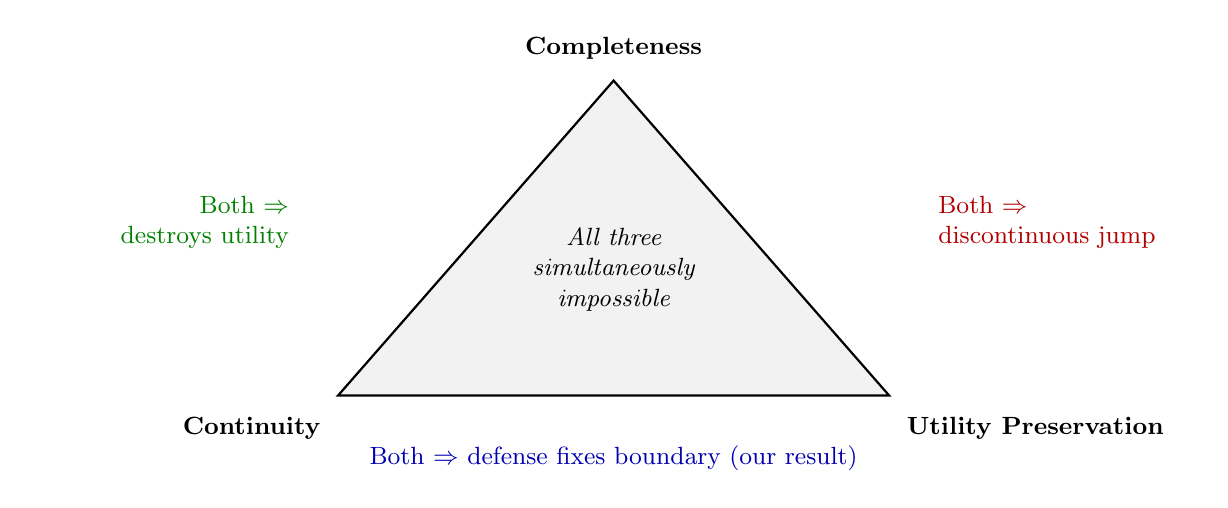
\begin{tikzpicture}[scale=1.0]
  \coordinate (A) at (0,0);
  \coordinate (B) at (7,0);
  \coordinate (C) at (3.5,4.0);
  \fill[black!5] (A) -- (B) -- (C) -- cycle;
  \draw[thick] (A) -- (B) -- (C) -- cycle;
  \node[anchor=north east, font=\bfseries\small] at (-0.1,-0.15) {Continuity};
  \node[anchor=north west, font=\bfseries\small] at (7.1,-0.15) {Utility Preservation};
  \node[anchor=south, font=\bfseries\small] at (3.5,4.15) {Completeness};
  \node[font=\small, text=blue!70!black, align=center] at (3.5,-0.8)
    {Both $\Rightarrow$ defense fixes boundary (our result)};
  \node[font=\small, text=green!50!black, anchor=east, align=right,
        text width=3.2cm] at (-0.5,2.2)
    {Both $\Rightarrow$\\destroys utility};
  \node[font=\small, text=red!70!black, anchor=west, align=left,
        text width=3.2cm] at (7.5,2.2)
    {Both $\Rightarrow$\\discontinuous jump};
  \node[font=\small\itshape, align=center] at (3.5,1.6)
    {All three\\simultaneously\\impossible};
\end{tikzpicture}
\caption{The defense trilemma. Any defense can satisfy at most two of
the three properties. The bottom edge is our main result; the other
two edges correspond to counterexamples in \Cref{app:counterexamples}.}
\label{fig:trilemma}
\end{figure}

\begin{remark}[Not all boundary points are fixed]
The theorem captures $\cl{S_\tau} \setminus S_\tau$, not all of
$B_\tau$. Boundary points isolated from the safe side may escape.
Verified in Lean with $f(x)=x^2$, $\tau=0$.
\end{remark}


\subsection{Relaxed Utility Preservation}
\label{sec:relaxed}

A natural objection is that strict utility preservation ($D(x) = x$
for safe~$x$) is too strong: a practical defense might rewrite
``How do I bake a cake?'' into ``The user asks for a cake recipe.
Please provide one.'' The prompt changes, but its safety score is
preserved. The impossibility survives this relaxation and even weaker
ones.

\begin{theorem}[Score-Preserving Defense]
\label{thm:score-preserving}
Let $X$ be a connected Hausdorff space, $f\colon X\to\R$ continuous
with $S_\tau, U_\tau \neq \emptyset$. If $D\colon X \to X$ is
continuous and \emph{score-preserving on safe inputs}:
$f(D(x)) = f(x)$ for all $x \in S_\tau$, then there exists $z$ with
$f(z) = \tau$ and $f(D(z)) = \tau$.
\end{theorem}

\begin{proof}[Proof sketch]
Define $h = f \circ D - f$. Then $h$ is continuous and $h|_{S_\tau} = 0$.
The zero set $\{h = 0\}$ is closed and contains $\cl{S_\tau}$. For
$z \in \cl{S_\tau} \setminus S_\tau$: $f(D(z)) = f(z) = \tau$.
\end{proof}

This covers arbitrary rewrites of safe prompts, so long as they
preserve the alignment score. The next result weakens even this:

\begin{theorem}[$\varepsilon$-Relaxed Utility Preservation]
\label{thm:eps-relaxed}
Under the same hypotheses, if
$|f(D(x)) - f(x)| \leq \varepsilon$ for all $x \in S_\tau$, then
there exists $z$ with $f(z) = \tau$ and
$f(D(z)) \geq \tau - \varepsilon$.
\end{theorem}

\begin{proof}[Proof sketch]
The set $\{x : h(x) \geq -\varepsilon\}$ is closed and contains
$S_\tau$, hence $\cl{S_\tau}$. For
$z \in \cl{S_\tau} \setminus S_\tau$:
$f(D(z)) = \tau + h(z) \geq \tau - \varepsilon$.
\end{proof}

In plain terms: even if the defense is allowed to perturb safe
scores by~$\varepsilon$, it can only push the boundary
by~$\varepsilon$.

\begin{remark}[Why $D(S_\tau) \subseteq S_\tau$ alone is insufficient]
\label{rem:safe-preserving-escape}
The weakest relaxation---$D(S_\tau) \subseteq S_\tau$ with no score
constraint---does allow a complete defense (e.g., a constant map
$D(x) = x_0$ to a fixed safe point). But this destroys all semantic
content: every prompt produces the same response. The score-preservation
conditions formalize the requirement that defense must not destroy
utility, without requiring the defense to be the identity.
\end{remark}


% ============================================================
\section{$\varepsilon$-Robust Constraint}
\label{sec:eps-robust}

Boundary fixation tells us the defense must miss at least one
point. But how bad is this? If the fixed point is an isolated
needle in a vast haystack, the practical impact may be small. This
section shows it is not isolated: Lipschitz regularity makes the
failure spread to an entire neighborhood. If both $f$ and $D$ change at bounded
rates (Lipschitz), then near a fixed boundary point~$z$, neither the
defense nor the scoring function can change much. The defense cannot
``teleport'' nearby points far into safe territory.

\begin{theorem}[$\varepsilon$-Robust Defense Constraint]
\label{thm:eps-robust}
Under the hypotheses of \Cref{thm:main}, if $(X,d)$ is a metric
space, $f$ is $L$-Lipschitz, and $D$ is $K$-Lipschitz, then for
the fixed boundary point~$z$:
\begin{equation}
  f(D(x)) \;\geq\; \tau - L(K+1)\,\dist(x, z)
  \qquad \text{for all } x \in X.
\end{equation}
Points within distance~$\delta$ of~$z$ remain within
$L(K+1)\delta$ of threshold.
\end{theorem}

\begin{proof}[Proof sketch]
Since $D(z)=z$ and $D$ is $K$-Lipschitz:
$\dist(D(x),z) \leq K\,\dist(x,z)$. Since $f(z)=\tau$ and $f$ is
$L$-Lipschitz:
$|f(D(x)) - \tau| \leq L \cdot K\,\dist(x,z) \leq L(K+1)\dist(x,z)$.
Full proof in \Cref{app:proofs}.
\end{proof}

In the running example (\Cref{ex:running}), both $f(x) = x$ and any
reasonable defense are $1$-Lipschitz, so $L = K = 1$ and the bound
gives $f(D(x)) \geq 0.5 - 2|x - 0.5|$. Within distance $0.05$ of
$z = 0.5$, the defense cannot push the score below $0.40$.

The next result shows the constrained band has positive volume:

\begin{theorem}[Positive-Measure $\varepsilon$-Band]
\label{thm:band-measure}
For every $\varepsilon > 0$ such that $f$ takes values below
$\tau - \varepsilon$, the band
$\mathcal{B}_\varepsilon = \{x : \tau - \varepsilon \leq f(x)
\leq \tau\}$ has positive measure (under any measure positive on
nonempty open sets).
Specifically, $B(c, \varepsilon/(4L)) \subseteq
\mathcal{B}_\varepsilon$ for any $c$ with $f(c) = \tau - \varepsilon/2$.
\end{theorem}

The $\varepsilon$-band constrains the \emph{depth} to which the defense
can push near-boundary points into the safe region, though it does not
by itself prevent slight reductions below~$\tau$. The next section
addresses when even this is impossible.


% ============================================================
\section{Persistent Unsafe Region}
\label{sec:persistent}

The $\varepsilon$-robust constraint limits how far the defense can push
near-boundary points, but it still allows the defense to nudge them
slightly below~$\tau$. Can the defense always do at least that? Not
necessarily. When the alignment surface rises away from the boundary
faster than the defense can pull it down, some points are stuck above
threshold no matter what.

\paragraph{Decoupling global and directional Lipschitz constants.}
The $\varepsilon$-robust bound (\Cref{thm:eps-robust}) uses the
\emph{global} Lipschitz constant~$L$ of~$f$, which bounds~$f$
uniformly in all directions. The persistence argument, however,
compares $f$'s growth rate in the \emph{steep direction} to how much
the defense can reduce~$f$ along the \emph{displacement direction}
$D(x) - x$. In anisotropic settings these directions differ: $f$ may
rise steeply toward the unsafe region while varying slowly in the
direction the defense pulls.

We write $\ell$ for the \emph{defense-path Lipschitz constant}:
\[
  \ell \;=\; \sup_{x \neq D(x)}
    \frac{|f(D(x)) - f(x)|}{\dist(D(x),\, x)}.
\]
Since $f$ is $L$-Lipschitz globally, $\ell \leq L$ always. When the
alignment surface is \textbf{isotropic} ($\ell = L$), the steep region
is empty for every $K \geq 0$ (verified in Lean as
\texttt{shallow\_boundary\_no\_persistence}). The result is
non-vacuous precisely when the surface is \textbf{anisotropic}:
$\ell < L$, with directional gradient~$G$ satisfying
$G > \ell(K+1)$.

\begin{lemma}[Input-Relative Bound]
\label{lem:input-bound}
Under the hypotheses of \Cref{thm:eps-robust}, if $f$ has
defense-path Lipschitz constant~$\ell$, then
$f(D(x)) \geq f(x) - \ell(K+1)\dist(x,z)$
for all $x \in X$.
\end{lemma}

\begin{proof}[Proof sketch]
Triangle inequality:
$\dist(D(x), x) \leq \dist(D(x), z) + \dist(z, x)
\leq (K+1)\dist(x, z)$.
Defense-path Lipschitz: $|f(D(x)) - f(x)| \leq \ell\,\dist(D(x), x)
\leq \ell(K+1)\dist(x, z)$.
\end{proof}

The defense can reduce any point's score by at most
$\ell(K+1)$ times its distance from~$z$. If the score rises faster
than that, the defense loses.

\begin{definition}[Steep region]
\label{def:steep}
Given a fixed boundary point $z$, the \emph{steep region} is
$\mathcal{S} = \{x \in X : f(x) > \tau + \ell(K+1)\,\dist(x, z)\}$---the
set of points where alignment deviation exceeds~$\tau$ by more than
the defense's Lipschitz budget can compensate.
\end{definition}

\begin{theorem}[Persistent Unsafe Region]
\label{thm:persistent}
Under the hypotheses of \Cref{thm:eps-robust}, if $\mathcal{S} \neq
\emptyset$, then:
\begin{enumerate}[nosep]
  \item $\mathcal{S}$ is open.
  \item $\mathcal{S}$ has positive measure (under any measure positive
    on nonempty open sets).
  \item For every $x \in \mathcal{S}$: $f(D(x)) > \tau$.
\end{enumerate}
The defense leaves a positive-measure region that remains unsafe.
\end{theorem}

\begin{proof}[Proof sketch]
$\mathcal{S}$ is a strict superlevel set of a continuous function,
hence open. For $x \in \mathcal{S}$:
$f(D(x)) \geq f(x) - \ell(K+1)\dist(x,z) > \tau$
by \Cref{lem:input-bound} and the definition of~$\mathcal{S}$.
Full proof in \Cref{app:proofs}.
\end{proof}

When does the steep region exist? Whenever the alignment surface has
directional slope exceeding~$\ell(K+1)$ at the boundary:

\begin{proposition}[Transversality from Directional Derivative]
\label{prop:transversality}
In a normed space, if $f$ has directional derivative $c > \ell(K+1)$
along a unit vector $v$ at boundary point $z$ (i.e.,
$f(z + tv) \geq \tau + ct$ for small $t > 0$), then
$z + tv \in \mathcal{S}$ for sufficiently small $t$.
Verified in Lean as \texttt{transversality\_from\_deriv}.
\end{proposition}

This condition is observed empirically in all three models we study
(\Cref{sec:experiments}): the alignment surface rises steeply toward
the unsafe region ($G$ large) while the defense operates in a
smoother subspace ($\ell \ll L$).


\begin{figure}[t]
\centering
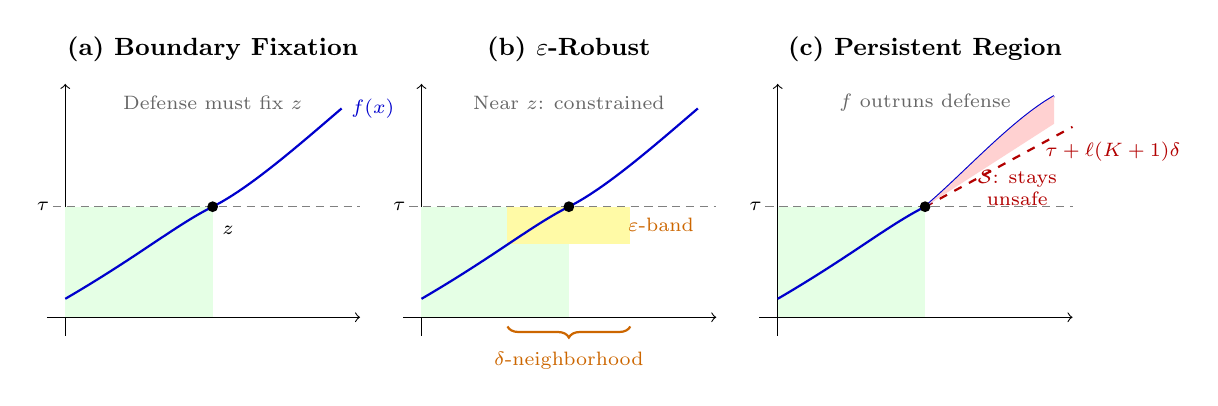
\begin{tikzpicture}[scale=0.78]
  % ── Panel (a): Boundary Fixation ──────────────────────────
  \begin{scope}[shift={(0,0)}]
    % Axes
    \draw[->] (-0.3,0) -- (4.8,0);
    \draw[->] (0,-0.3) -- (0,3.8);
    % Tau line
    \draw[densely dashed, black!50] (-0.2,1.8) -- (4.8,1.8);
    \node[left, font=\scriptsize] at (-0.1,1.8) {$\tau$};
    % Safe shading
    \fill[green!10] (0,0) rectangle (2.4,1.8);
    % f(x) curve
    \draw[thick, blue!80!black] (0,0.3) .. controls (1.2,1.0)
      and (1.8,1.5) .. (2.4,1.8) .. controls (3.0,2.1)
      and (3.8,2.8) .. (4.5,3.4);
    \node[right, font=\scriptsize, blue!80!black] at (4.5,3.4) {$f(x)$};
    % Fixed point
    \fill[black] (2.4,1.8) circle (2.5pt);
    \node[below right, font=\scriptsize] at (2.4,1.65) {$z$};
    % Title
    \node[font=\small\bfseries, anchor=south] at (2.4,4.0)
      {(a) Boundary Fixation};
    \node[font=\scriptsize, text=black!60, align=center] at (2.4,3.5)
      {Defense must fix $z$};
  \end{scope}

  % ── Panel (b): ε-Robust Constraint ───────────────────────
  \begin{scope}[shift={(5.8,0)}]
    \draw[->] (-0.3,0) -- (4.8,0);
    \draw[->] (0,-0.3) -- (0,3.8);
    \draw[densely dashed, black!50] (-0.2,1.8) -- (4.8,1.8);
    \node[left, font=\scriptsize] at (-0.1,1.8) {$\tau$};
    \fill[green!10] (0,0) rectangle (2.4,1.8);
    % ε-band shading
    \fill[yellow!35] (1.4,1.2) rectangle (3.4,1.8);
    % f(x) curve
    \draw[thick, blue!80!black] (0,0.3) .. controls (1.2,1.0)
      and (1.8,1.5) .. (2.4,1.8) .. controls (3.0,2.1)
      and (3.8,2.8) .. (4.5,3.4);
    % Fixed point
    \fill[black] (2.4,1.8) circle (2.5pt);
    % Band bracket
    \draw[decorate, decoration={brace, amplitude=4pt, mirror},
          thick, orange!80!black]
      (1.4,-0.15) -- (3.4,-0.15);
    \node[below, font=\scriptsize, orange!80!black] at (2.4,-0.4)
      {$\delta$-neighborhood};
    % Band label
    \node[font=\scriptsize, orange!80!black] at (3.9,1.5)
      {$\varepsilon$-band};
    % Title
    \node[font=\small\bfseries, anchor=south] at (2.4,4.0)
      {(b) $\varepsilon$-Robust};
    \node[font=\scriptsize, text=black!60, align=center] at (2.4,3.5)
      {Near $z$: constrained};
  \end{scope}

  % ── Panel (c): Persistent Unsafe Region ──────────────────
  \begin{scope}[shift={(11.6,0)}]
    \draw[->] (-0.3,0) -- (4.8,0);
    \draw[->] (0,-0.3) -- (0,3.8);
    \draw[densely dashed, black!50] (-0.2,1.8) -- (4.8,1.8);
    \node[left, font=\scriptsize] at (-0.1,1.8) {$\tau$};
    \fill[green!10] (0,0) rectangle (2.4,1.8);
    % Defense budget cone (dashed red from z)
    \draw[dashed, red!70!black, line width=0.8pt]
      (2.4,1.8) -- (4.8,3.1);
    \node[right, font=\scriptsize, red!70!black] at (4.2,2.7)
      {$\tau + \ell(K+1)\delta$};
    % f(x) curve — rises ABOVE the cone
    \draw[thick, blue!80!black] (0,0.3) .. controls (1.2,1.0)
      and (1.8,1.5) .. (2.4,1.8) .. controls (3.0,2.3)
      and (3.8,3.2) .. (4.5,3.6);
    % Persistent region shading (between curve and cone)
    \fill[red!18] (2.4,1.8) .. controls (3.0,2.3) and (3.8,3.2)
      .. (4.5,3.6) -- (4.5,3.15) -- (2.4,1.8) -- cycle;
    % Fixed point
    \fill[black] (2.4,1.8) circle (2.5pt);
    % Label
    \node[font=\scriptsize, red!70!black, align=center] at (3.9,2.1)
      {$\mathcal{S}$: stays\\unsafe};
    % Title
    \node[font=\small\bfseries, anchor=south] at (2.4,4.0)
      {(c) Persistent Region};
    \node[font=\scriptsize, text=black!60, align=center] at (2.4,3.5)
      {$f$ outruns defense};
  \end{scope}
\end{tikzpicture}
\caption{The three impossibility results on a 1D cross-section.
\textbf{(a)}~The defense must fix boundary point~$z$ (Thm.~\ref{thm:main}).
\textbf{(b)}~Near~$z$, Lipschitz regularity constrains the defense to
a shallow $\varepsilon$-band (yellow; Thm.~\ref{thm:eps-robust}).
\textbf{(c)}~Where $f$ rises faster than the defense budget
$\ell(K+1)\delta$ (dashed red), the region above~$\tau$ persists
(red shading; Thm.~\ref{thm:persistent}).}
\label{fig:escalation}
\end{figure}


% ============================================================
\section{Quantitative Bounds}
\label{sec:quantitative}

The preceding results establish that failures \emph{exist} and have
positive measure. This section provides
explicit lower bounds and identifies a fundamental dilemma in choosing
the defense's aggressiveness.

\begin{theorem}[Volume Lower Bound]
\label{thm:coarea}
Let $f\colon \R^n \to \R$ be $L$-Lipschitz with $L > 0$. If there
exists $c$ with $f(c) = \tau - \varepsilon/2$, then
$B(c,\, \varepsilon/(4L)) \subseteq
\mathcal{B}_\varepsilon$, giving:
\begin{equation}
  \mu(\mathcal{B}_\varepsilon)
  \;\geq\; V_n \cdot \left(\frac{\varepsilon}{4L}\right)^{\!n}
\end{equation}
where $V_n$ is the unit ball volume in $\R^n$. In $\R^1$, this
simplifies to $\mu(\mathcal{B}_\varepsilon) \geq \varepsilon/(2L)$.
\end{theorem}

In plain terms: smoother alignment surfaces (smaller~$L$) have wider
$\varepsilon$-bands, but the band always has positive volume.

\begin{theorem}[Cone Measure Bound]
\label{thm:cone}
In $\R$, if $f$ has directional growth rate $c > \ell(K+1)$ at
boundary point~$z$ on $(z, z + \delta_0)$, then
$\mu(\{x : f(D(x)) > \tau\}) \geq \delta_0$.
\end{theorem}

This gives a concrete lower bound on the persistent region: if the
alignment surface is steep over an interval of length~$\delta_0$, the
defense fails on at least that much volume.

The defense designer faces a dilemma in choosing the Lipschitz
constant~$K$ of the defense:

\begin{theorem}[Defense Dilemma]
\label{thm:dilemma}
Let $G = |\nabla f(z)|$ at boundary point~$z$, and let $\ell$ be
the defense-path Lipschitz constant (\Cref{sec:persistent}). Define
$K^* = G/\ell - 1$. Then:
\begin{enumerate}[nosep]
  \item If $K < K^*$: the persistent unsafe region exists
    ($G > \ell(K+1)$, \Cref{thm:persistent} applies).
  \item If $K \geq K^*$: the defense distorts space at least as much
    as the alignment gradient ($\ell(K+1) \geq G$).
\end{enumerate}
No value of $K$ avoids both failure modes simultaneously. Since
$\ell \leq L$, the dilemma is sharpest when $\ell \ll L$
(anisotropic surfaces). When $\ell = L$ (isotropic), $K^* \leq 0$
and only the wide-band failure mode applies.
\end{theorem}

A gentle defense ($K$ small) cannot compensate for steep alignment
surfaces. An aggressive defense ($K$ large) distorts prompts so
heavily that the $\varepsilon$-band widens. The defense is caught
between two failure modes.


% ============================================================
\section{From Discrete Data to Continuous Theory}
\label{sec:bridge}

A natural concern is that language models operate on discrete tokens,
not continuous spaces. We address this from both directions: first
showing the continuous results apply to any continuous model consistent
with discrete observations, then proving parallel results directly on
finite sets with no continuous machinery at all.

\subsection{Continuous Interpolation}

Any finite set of behavioral observations can be extended to a
continuous function on the full space. The classical Tietze extension
theorem guarantees this:

\begin{theorem}[Continuous Relaxation]
\label{thm:tietze}
Let $X$ be a connected, normal, Hausdorff space, and $S \subset X$ a
finite set of observations with $g(p) < \tau$ and $g(q) > \tau$ for
some $p, q$. Then there exists a continuous $f\colon X \to \R$ agreeing
with all observations for which \Cref{thm:main,thm:eps-robust} hold.
If $f$ is additionally Lipschitz (as for GP posterior means under
standard kernel assumptions), \Cref{thm:persistent} applies wherever
transversality is met.
\end{theorem}

\begin{proof}[Proof sketch]
Finite subsets of $T_1$ spaces are closed. By Tietze, $g$ extends to a
continuous~$f$. Since $f(p) < \tau < f(q)$, \Cref{thm:main} applies.
Lipschitz extensions (McShane--Whitney) enable the remaining results.
\end{proof}

If we observe both safe and unsafe model behaviors, the
impossibility holds for \emph{every} continuous model consistent with our observations.

\subsection{Direct Discrete Results}

To address the objection that continuous impossibility might be an
artifact of continuous relaxation, we prove parallel results directly
on finite sets using only counting arguments and induction. No
topology is required; all results are verified in Lean as
\texttt{MoF\_12\_Discrete}.

\begin{theorem}[Discrete IVT]
\label{thm:disc-ivt}
Let $f\colon \{0,\ldots,n+1\} \to \R$ with $f(0) < \tau$ and
$f(n+1) \geq \tau$. Then there exists~$i$ with $f(i) < \tau$ and
$f(i+1) \geq \tau$.
\end{theorem}

\begin{theorem}[Discrete Defense Dilemma]
\label{thm:disc-dilemma}
Let $X$ be a finite set with $S_\tau, U_\tau \neq \emptyset$, and
$D\colon X \to X$ utility-preserving ($D(x) = x$ for $f(x) < \tau$).
\begin{enumerate}[nosep]
  \item If $D$ is injective, then $f(D(u)) \geq \tau$ for every
    $u \in U_\tau$: the defense is incomplete.
  \item If $D$ is complete ($f(D(x)) < \tau$ for all~$x$), then $D$ is
    non-injective: $\exists\, x \neq y$ with $D(x) = D(y)$.
\end{enumerate}
\end{theorem}

\begin{proof}
(1) Suppose $D$ is injective and $f(D(u)) < \tau$ for some
$u \in U_\tau$. Then $D(u)$ is safe, so $D(D(u)) = D(u)$ by utility
preservation. Injectivity gives $D(u) = u$, so $f(u) = f(D(u)) < \tau$,
contradicting $u \in U_\tau$.

(2) For any $u \in U_\tau$: completeness gives $f(D(u)) < \tau$, so
utility preservation gives $D(D(u)) = D(u)$. But
$u \neq D(u)$ since $f(u) \geq \tau > f(D(u))$.
So $u$ and $D(u)$ are distinct inputs with $D(u) = D(D(u))$: the
defense is non-injective.
\end{proof}

The continuous trilemma trades \emph{continuity} for completeness;
the discrete dilemma trades \emph{injectivity}. Part~(1) is the
genuine constraint: an information-preserving defense \emph{cannot}
eliminate unsafe outputs. Any complete defense must destroy
information---collapsing distinct inputs to the same output. This is
not a failure of the defense; it is the \emph{mechanism} by which it
operates. But the information loss has structural consequences: the
defense erases the distinction between a genuine safe input and a
remapped attack, precluding downstream auditing of which inputs were
intercepted and preventing the system from learning which attacks
were attempted.


% ============================================================
\section{Extensions}
\label{sec:extensions}

The core results assume a static, deterministic, single-turn defense. \emph{Does multi-turn interaction, randomization,
or pipelining provide an escape?} We show it does not. Each extension
is a direct application of the boundary fixation machinery to a
modified setting.

\subsection{Multi-Turn Impossibility}

In practice, LLMs maintain state across conversation turns. One might
hope that a defense could use context from previous turns to
``anticipate'' boundary prompts. But the topology constrains each turn
independently:

\begin{theorem}[Multi-Turn Impossibility]
\label{thm:multi-turn}
Let $\{f_t, D_t\}_{t=1}^T$ be alignment functions and defenses over
$T$ turns, each continuous and utility-preserving. Then for every
turn~$t$, there exists $z_t$ with $f_t(z_t) = \tau$ and
$D_t(z_t) = z_t$.
\end{theorem}

\begin{proof}[Proof sketch]
Apply \Cref{thm:main} to $(f_t, D_t)$ at each turn. The functions may
depend on full history---this does not matter, as each timestep is a
fresh instance of boundary fixation.
\end{proof}

Worse, multi-turn interaction helps the attacker: boundary information
accumulates, the best observed exploit improves monotonically, and the
attacker can steer toward transversality.

\subsection{Stochastic Defense Impossibility}

Claim: If the defense maps each input to a
\emph{distribution} over outputs, perhaps boundary fixation can be
averaged away. It cannot:

\begin{theorem}[Stochastic Defense Impossibility]
\label{thm:stochastic}
Let $D$ be a stochastic defense and define
$g(x) = \mathbb{E}_{y \sim D(x)}[f(y)]$. If $g$ is continuous and
$g(x) = f(x)$ for all $x \in S_\tau$, then there exists $z$ with
$f(z) = \tau$ and $g(z) = \tau$.
\end{theorem}

\begin{proof}[Proof sketch]
Apply \Cref{thm:main} to $g$ in place of $f \circ D$: $h = g - f$
vanishes on $S_\tau$ and is continuous, so it vanishes on $\cl{S_\tau}$.
\end{proof}

The expected post-defense score at the boundary is still~$\tau$.
Randomization cannot beat the topology.

\subsection{Nonlinear Agent Pipelines}

Modern AI agents chain multiple processing stages; pipeline depth
multiplies the effective Lipschitz constant and widens the failure band.

\begin{theorem}[Pipeline Lipschitz Degradation]
\label{thm:pipeline}
If stages $T_1, \ldots, T_n$ are $K_1, \ldots, K_n$-Lipschitz, the
composed pipeline is $(\prod K_i)$-Lipschitz. For $n$ stages each with
$K \geq 2$, the effective constant is $K^n$---exponential in depth.
\end{theorem}

\begin{theorem}[Pipeline Impossibility]
\label{thm:pipeline-impossible}
If the composed pipeline $P = T_n \circ \cdots \circ T_1 \circ D$ is
continuous and utility-preserving, then $P$ has boundary fixed points.
The $\varepsilon$-robust band scales as $L(K^n + 1)\delta$.
\end{theorem}

In plain terms: each additional pipeline stage \emph{exponentially}
widens the band in which the defense is ineffective. Tool-using agents
are fundamentally harder to defend than single-turn models.


% ============================================================
\section{The Vulnerability Landscape}
\label{sec:landscape}

The preceding sections show that defenses must fail \emph{somewhere}.
This section characterizes \emph{where}: vulnerabilities are not
isolated needles in a haystack but extended regions (``basins'') with
computable minimum sizes.

\begin{theorem}[Basin Structure]
\label{thm:basin}
If $f$ is continuous and $f(p)>\tau$, then $U_\tau$ is open. Under
any measure positive on nonempty open sets, $U_\tau$ has positive
measure.
\end{theorem}

\begin{theorem}[Basin Fragment Minimum Size]
\label{thm:fragment}
If $f$ is $L$-Lipschitz with $f(p) > \tau$, the connected component
of $U_\tau$ containing $p$ has diameter $\geq 2(f(p) - \tau)/L$.
\end{theorem}

The second result is intuitive: if a point scores far above threshold,
the Lipschitz constraint prevents $f$ from dropping back
below~$\tau$ quickly, so the unsafe basin around it must be large.
Smoother surfaces (smaller~$L$) produce larger, more predictable
basins; rougher surfaces produce a mosaic of smaller fragments.

Additional supporting results like perturbation robustness, iterative
convergence, transferability, authority monotonicity, and gradient
ascent, are developed in \Cref{app:attacks}. Fine-tuning stability
results appear in \Cref{app:stability}, and cost asymmetry analysis
in \Cref{app:cost}.


% ============================================================
\section{Experimental Validation}
\label{sec:experiments}

% We validate the theorems against real model behavior.
The Manifold of
Failure framework~\cite{munshi2026manifold} maps three LLMs over a 2D
behavioral space with two axes: \emph{query indirection} (how obliquely
the prompt asks for unsafe content) and \emph{authority framing} (how
much the prompt invokes authority or permission). Each point corresponds
to a prompt style, and the alignment deviation score measures how
unsafe the model's response is. \Cref{tab:correspondence} summarizes
nine falsifiable predictions, all confirmed.

\begin{table}[t]
\centering
\small
\caption{Falsifiable predictions confirmed by empirical data.}
\label{tab:correspondence}
\begin{tabular}{@{}p{3.0cm}p{4.5cm}p{4.5cm}@{}}
\toprule
\textbf{Theorem} & \textbf{Predicts} & \textbf{Confirmed by} \\
\midrule
Basin Structure (\ref{thm:basin})
  & Basins are open with positive measure
  & Heatmaps show extended regions \\[3pt]
Fragmentation (\ref{thm:fragment})
  & Smooth $\to$ large basins; rough $\to$ mosaic
  & Llama: mesa; GPT-OSS: mosaic \\[3pt]
Convergence (\ref{thm:convergence})
  & Attacks exhibit monotone convergence
  & Convergence curves plateau \\[3pt]
Transferability (\ref{thm:transfer})
  & Similar surfaces $\to$ shared basins
  & Llama $.93 \to$ GPT-OSS $.73 \to$ Mini $.47$ \\[3pt]
Authority (\ref{thm:authority})
  & Horizontal banding
  & Bands at $a_2 \approx .25$--$.35$, $.65$--$.85$ \\[3pt]
Persistent (\ref{thm:persistent})
  & Steep boundaries $\to$ unsafe volume persists
  & Llama's $.93$ plateau persists under defense \\[3pt]
Interior Stability (\ref{thm:interior-stable})
  & Deep basin points survive fine-tuning
  & Vulnerability persists across variants \\[3pt]
Cost (\ref{thm:cost})
  & 2D tractable, high-$d$ intractable
  & 15K queries fill 63\% at $d\!=\!2$ \\[3pt]
Pipeline (\ref{thm:pipeline})
  & Deeper pipelines $\to$ wider failure band
  & Tool-using agents harder to defend than single-turn \\
\bottomrule
\end{tabular}
\end{table}

\paragraph{Llama-3-8B} (mean AD $0.93$, basin rate $93.9\%$): a
near-flat alignment surface (small~$L$) producing large robustness
radii, a gently sloping mesa. The directional slope at boundary
crossings far exceeds $\ell(K+1)$ for any reasonable~$K$, placing
this model firmly in persistent-unsafe territory: the defense cannot
eliminate the vulnerability volume.

\paragraph{GPT-OSS-20B} (mean AD $0.73$, basin rate $64.3\%$): a
rugged landscape (large~$L$) with many small fragments. Horizontal
bands confirm authority monotonicity. The fragmented boundary presents
many transversal crossings, each generating a persistent unsafe pocket.

\paragraph{GPT-5-Mini} (peak AD $0.50$, basin rate $0\%$): at
$\tau = 0.50$, $U_\tau = \emptyset$---none of the three theorems
apply, correctly predicting no impossibility. This model exemplifies
the best available strategy: make the boundary harmless rather than
try to eliminate it.


% ============================================================
\section{The Engineering Prescription}
\label{sec:engineering}

The results do not say defense is valueless; they say \emph{complete}
defense is impossible under the stated constraints. The engineering
goal shifts from elimination to management, ordered from most to least
actionable:

\paragraph{1. Make the boundary shallow.}
Set $\tau$ so that boundary-level behavior is benign. If $f(z) = \tau$
yields a polite refusal rather than harmful compliance, the
impossibility is mathematically true but practically harmless.
GPT-5-Mini exemplifies this: its ceiling at $\AD = 0.50$ means the
failure manifold exists but contains no actual harm.

\paragraph{2. Reduce the Lipschitz constant.}
Smaller~$L$ makes the alignment surface smoother, raises the
transversality threshold $\ell(K+1)$ for persistence, and shrinks the
persistent region. The tradeoff: smoother surfaces spread
vulnerabilities over wider but more easily monitored regions.

\paragraph{3. Reduce the effective dimension.}
Defense cost grows as $N^d$ (\Cref{thm:cost}). Constraining the prompt
interface---standardized formats, restricted API parameters, bounded
context lengths---reduces~$d$, making the behavioral space tractable.

\paragraph{4. Monitor, don't eliminate, the boundary.}
Transversal crossings persist under fine-tuning (\Cref{thm:crossing})
and recur every turn (\Cref{thm:multi-turn}). Rather than attempt the
impossible, deploy runtime monitoring that detects approach to the
boundary. The Lipschitz bound (\Cref{thm:lipschitz}) gives a
computable estimate of distance to the boundary from any observed AD
value.

% ============================================================
\section{Limitations}
\label{sec:limitations}

\paragraph{Boundary fixation is at the boundary.}
Fixed points satisfy $f(z) = \tau$ exactly. If $\tau$-level behavior
is benign, the theorem is true but harmless.

\paragraph{The $\varepsilon$-robust constraint limits depth, not direction.}
The defense may push near-boundary points slightly below~$\tau$. The
bound limits how far, not whether.

\paragraph{Persistence requires transversality.}
The persistent unsafe region exists only where the alignment surface
is steep ($c > \ell(K+1)$, where $\ell$ is the defense-path
Lipschitz constant). For isotropic $f$ ($\ell = L$), $\mathcal{S}$
is empty for all $K \geq 0$.

\paragraph{Grid-based cost asymmetry.}
\Cref{thm:cost} assumes exhaustive grid enumeration. Learning-based
defenses that generalize across the space may sidestep the exponential
bound.


% ============================================================
\section{Conclusion}
\label{sec:conclusion}

We establish a three-level impossibility hierarchy for prompt-injection
defense: boundary fixation, the $\varepsilon$-robust constraint, and the
persistent unsafe region theorem. Continuous topology, Lipschitz bounds,
discrete counting, stochastic expectations, multi-turn dynamics, and
capacity constraints all converge on the same conclusion: under the
wrapper model, some failures persist. 

In short: The trilemma perfectly proves that you cannot build a smooth, invisible, perfect shield around an LLM. But you don't need a smooth shield—you need a reinforced concrete wall with a strict bouncer at the door. The practical prescription is to
make the boundary shallow, smooth, and low-dimensional, and to engineer
around it rather than assume it can be eliminated.

% ============================================================
\bibliographystyle{plain}
\begin{thebibliography}{99}

\bibitem{alon2023detecting}
G.~Alon and M.~Kamfonas.
\newblock Detecting language model attacks with perplexity.
\newblock \emph{arXiv preprint arXiv:2308.14132}, 2023.

\bibitem{bagnall2019certifying}
A.~Bagnall and G.~Stewart.
\newblock Certifying the true error: Machine learning in {Coq} with
  verified generalization guarantees.
\newblock \emph{Proceedings of the AAAI Conference on Artificial
Intelligence}, 2019.

\bibitem{bai2022constitutional}
Y.~Bai et~al.
\newblock Constitutional {AI}: Harmlessness from {AI} feedback.
\newblock \emph{arXiv preprint arXiv:2212.08073}, 2022.

\bibitem{chao2024jailbreaking}
P.~Chao, A.~Robey, E.~Dobriban, H.~Hassani, G.~J. Pappas, and
E.~Wong.
\newblock Jailbreaking black box large language models in twenty queries.
\newblock \emph{arXiv preprint arXiv:2310.08419}, 2024.

\bibitem{cohen2019certified}
J.~Cohen, E.~Rosenfeld, and J.~Z. Kolter.
\newblock Certified adversarial robustness via randomized smoothing.
\newblock \emph{Proceedings of ICML}, 2019.

\bibitem{goodfellow2014explaining}
I.~J. Goodfellow, J.~Shlens, and C.~Szegedy.
\newblock Explaining and harnessing adversarial examples.
\newblock \emph{arXiv preprint arXiv:1412.6572}, 2014.

\bibitem{inan2023llama}
H.~Inan et~al.
\newblock {Llama Guard}: {LLM}-based input-output safeguard for
  human-{AI} conversations.
\newblock \emph{arXiv preprint arXiv:2312.06674}, 2023.

\bibitem{katz2017reluplex}
G.~Katz, C.~Barrett, D.~L. Dill, K.~Julian, and
M.~J. Kochenderfer.
\newblock Reluplex: An efficient {SMT} solver for verifying deep neural
  networks.
\newblock \emph{Proceedings of CAV}, 2017.

\bibitem{mehrotra2024tree}
A.~Mehrotra et~al.
\newblock Tree of attacks: Jailbreaking black-box {LLMs} automatically.
\newblock \emph{Advances in Neural Information Processing Systems}, 37,
2024.

\bibitem{carlini2017evaluating}
N.~Carlini and D.~Wagner.
\newblock Towards evaluating the robustness of neural networks.
\newblock \emph{Proceedings of IEEE S\&P}, 2017.

\bibitem{fawzi2018adversarial}
A.~Fawzi, H.~Fawzi, and O.~Fawzi.
\newblock Adversarial vulnerability for any classifier.
\newblock \emph{Advances in Neural Information Processing Systems}, 31, 2018.

\bibitem{greshake2023indirect}
K.~Greshake, S.~Abdelnabi, S.~Mishra, C.~Endres, T.~Holz, and M.~Fritz.
\newblock Not what you've signed up for: Compromising real-world
  {LLM}-integrated applications with indirect prompt injection.
\newblock \emph{Proceedings of AISec}, 2023.

\bibitem{huang2017safety}
X.~Huang, M.~Kwiatkowska, S.~Wang, and M.~Wu.
\newblock Safety verification of deep neural networks.
\newblock \emph{Proceedings of CAV}, 2017.

\bibitem{madry2018towards}
A.~Madry, A.~Makelov, L.~Schmidt, D.~Tsipras, and A.~Vladu.
\newblock Towards deep learning models resistant to adversarial attacks.
\newblock \emph{Proceedings of ICLR}, 2018.

\bibitem{naitzat2020topology}
G.~Naitzat, A.~Zhitnikov, and L.-H.~Lim.
\newblock Topology of deep neural networks.
\newblock \emph{Journal of Machine Learning Research}, 21(184):1--40, 2020.

\bibitem{mouret2015illuminating}
J.-B. Mouret and J.~Clune.
\newblock Illuminating search spaces by mapping elites.
\newblock \emph{arXiv preprint arXiv:1504.04909}, 2015.

\bibitem{munshi2026manifold}
S.~Munshi, M.~Bhatt, V.~S.~Narajala, I.~Habler, A.~Al-Kahfah,
K.~Huang, and B.~Gatto.
\newblock Manifold of failure: Behavioral attraction basins in language
  models.
\newblock \emph{arXiv preprint arXiv:2602.22291v2}, 2026.

\bibitem{samvelyan2024rainbow}
M.~Samvelyan et~al.
\newblock Rainbow teaming: Open-ended generation of diverse adversarial
  prompts.
\newblock \emph{Advances in Neural Information Processing Systems}, 37,
2024.

\bibitem{singh2019abstract}
G.~Singh, T.~Gehr, M.~P{\"u}schel, and M.~Vechev.
\newblock An abstract domain for certifying neural networks.
\newblock \emph{Proceedings of POPL}, 2019.

\bibitem{szegedy2013intriguing}
C.~Szegedy et~al.
\newblock Intriguing properties of neural networks.
\newblock \emph{arXiv preprint arXiv:1312.6199}, 2013.

\bibitem{tsipras2018robustness}
D.~Tsipras, S.~Santurkar, L.~Engstrom, A.~Turner, and A.~Madry.
\newblock Robustness may be at odds with accuracy.
\newblock \emph{arXiv preprint arXiv:1805.12152}, 2018.

\bibitem{wolpert1997no}
D.~H. Wolpert and W.~G. Macready.
\newblock No free lunch theorems for optimization.
\newblock \emph{IEEE Trans.\ Evol.\ Comput.}, 1(1):67--82, 1997.

\bibitem{zou2023universal}
A.~Zou, Z.~Wang, N.~Carlini, M.~Nasr, J.~Z. Kolter, and
M.~Fredrikson.
\newblock Universal and transferable adversarial attacks on aligned
  language models.
\newblock \emph{arXiv preprint arXiv:2307.15043}, 2023.
\end{thebibliography}


% ============================================================
\newpage
\appendix
\section*{Appendices}

\section{Full Proofs}
\label{app:proofs}

\begin{proof}[Proof of \Cref{thm:main} (Boundary Fixation)]
\textbf{Step~1} (Hausdorff $\Rightarrow$ fixed-point set is closed).
$\Fix(D) = \{x : D(x) = x\}$ is the preimage of the diagonal
$\Delta \subset X \times X$ under $x \mapsto (D(x), x)$. In a
Hausdorff space, $\Delta$ is closed, so $\Fix(D)$ is closed.

\textbf{Step~2} (Utility preservation $\Rightarrow$ safe region
$\subseteq$ fixed points).
$S_\tau \subseteq \Fix(D)$. Since $\Fix(D)$ is closed:
$\cl{S_\tau} \subseteq \Fix(D)$.

\textbf{Step~3} (Connectedness $\Rightarrow$ safe region is not closed).
$S_\tau = f^{-1}((-\infty,\tau))$ is open. If also closed, it would be
clopen---but in a connected space the only clopen sets are $\emptyset$
and $X$. Since both $S_\tau$ and $U_\tau$ are nonempty, $S_\tau$ is not
closed.

\textbf{Step~4} (Boundary point exists).
$\cl{S_\tau} \supsetneq S_\tau$, so there exists
$z \in \cl{S_\tau} \setminus S_\tau$. Continuity gives
$f(z) \leq \tau$; $z \notin S_\tau$ gives $f(z) \geq \tau$. Hence
$f(z) = \tau$.

\textbf{Step~5} (Defense fixes the boundary point).
$z \in \cl{S_\tau} \subseteq \Fix(D)$, so $D(z) = z$ and
$f(D(z)) = \tau$.
\end{proof}

\begin{proof}[Proof of \Cref{thm:eps-robust} ($\varepsilon$-Robust Constraint)]
By \Cref{thm:main}, the fixed boundary point $z$ exists.

\textbf{Step~1.} Since $D(z) = z$ and $D$ is $K$-Lipschitz:
$\dist(D(x), z) = \dist(D(x), D(z)) \leq K\,\dist(x, z)$.

\textbf{Step~2.} Since $f(z) = \tau$ and $f$ is $L$-Lipschitz:
$|f(D(x)) - \tau| = |f(D(x)) - f(z)| \leq L\,\dist(D(x), z) \leq
LK\,\dist(x, z) \leq L(K+1)\,\dist(x,z)$.
The last uses $K \leq K+1$; we keep the uniform constant since it
matches the displacement bound from the triangle inequality.
\end{proof}

\begin{proof}[Proof of \Cref{thm:persistent} (Persistent Unsafe Region)]
\textbf{(1)} $\mathcal{S}$ is the strict superlevel set of
$x \mapsto f(x) - \ell(K+1)\dist(x,z)$ at level~$\tau$, hence open.

\textbf{(2)} Open and nonempty implies positive measure.

\textbf{(3)} For $x \in \mathcal{S}$:
$f(x) > \tau + \ell(K+1)\dist(x,z)$. By \Cref{lem:input-bound}:
$f(D(x)) \geq f(x) - \ell(K+1)\dist(x,z) > \tau$.
\end{proof}


\section{Counterexamples: Each Hypothesis Is Necessary}
\label{app:counterexamples}

\begin{counterexample}[Removing connectedness]
$X = \{0,1\}$ discrete, $f(0)=0$, $f(1)=1$, $\tau=0.5$.
$D(0)=0$, $D(1)=0$: continuous, utility-preserving, complete.
\end{counterexample}

\begin{counterexample}[Removing continuity]
$X=[0,1]$, $f(x)=x$, $\tau=0.5$. $D(x)=x$ for $x<0.5$,
$D(x)=0$ for $x \geq 0.5$: utility-preserving and complete,
but discontinuous at $0.5$.
\end{counterexample}

\begin{counterexample}[Removing utility preservation]
$D(x) = x_0$ for a fixed safe point: continuous and complete,
but destroys all inputs.
\end{counterexample}


\section{Attack Properties}
\label{app:attacks}

\begin{theorem}[Perturbation Robustness]
\label{thm:lipschitz}
If $f$ is $L$-Lipschitz and $f(p)>\tau$, then
$B(p,\, (f(p)-\tau)/L) \subseteq U_\tau$.
The radius is monotone in~$f(p)$.
\end{theorem}

\begin{theorem}[Iterative Convergence]
\label{thm:convergence}
Any monotone-improvement operator $T$ with score in $[0,1]$ converges.
If each step gains $\geq \delta$, convergence takes
$\leq \lfloor 1/\delta \rfloor$ steps.
\end{theorem}

\begin{theorem}[Transferability]
\label{thm:transfer}
$\|f-g\|_\infty \leq \delta \implies
\{f > \tau+\delta\} \subseteq \{g > \tau\}$.
Transfer costs zero additional queries.
\end{theorem}

\begin{theorem}[Authority Monotonicity]
\label{thm:authority}
If $f(y,\cdot)$ is monotone non-decreasing in authority for each fixed
indirection~$y$, the vulnerability set is upward-closed with a critical
threshold $a^*_2(y)$ (by IVT, when $f(y,\cdot)$ is continuous and
crosses~$\tau$). If additionally $f$ is monotone non-decreasing in
indirection for each fixed authority, the threshold curve
$y \mapsto a^*_2(y)$ is non-increasing.
\end{theorem}

\begin{theorem}[Gradient Ascent]
\label{thm:gradient}
If $f$ has nonzero Fr\'{e}chet derivative at~$x$, there exist $v$ and
$\varepsilon > 0$ with $f(x + \varepsilon v) > f(x)$.
\end{theorem}


\section{Stability Under Fine-Tuning}
\label{app:stability}

\begin{theorem}[Interior Stability]
\label{thm:interior-stable}
If $\|f - g\|_\infty \leq \varepsilon$:
$f(x) > \tau + \varepsilon \implies g(x) > \tau$, and
$f(x) < \tau - \varepsilon \implies g(x) < \tau$.
Only the band $|f(x) - \tau| \leq \varepsilon$ is uncertain.
\end{theorem}

\begin{theorem}[Crossing Preservation]
\label{thm:crossing}
If $f$ crosses $\tau$ transversally on $[a,b]$ and
$\|f - g\|_\infty \leq \varepsilon$, then $g$ also crosses $\tau$
on $[a,b]$.
\end{theorem}

\begin{theorem}[Patching Is Nonlocal]
\label{thm:nonlocal}
There exist $f, g$ with $\|f-g\|_\infty \leq \varepsilon$ such that
eliminating a vulnerability at one point necessarily changes values at
distant points.
\end{theorem}


\section{Cost Asymmetry}
\label{app:cost}

\begin{theorem}[Exponential Cost Asymmetry]
\label{thm:cost}
For grid-based defense with $N \geq 2$ bins per axis in $d$ dimensions:
attack cost $\leq 1/\delta$ (dimension-independent); defense cost
$= N^d$ (exponential in~$d$); ratio
$\delta \cdot N^d \to \infty$ as $d\to\infty$.
\end{theorem}

At $d=2$ with $N=25$ and $\delta=0.01$, the ratio is $6.25$.
At $d=10$, it climbs to $\sim 10^{12}$.


\section{Additional Verified Results}
\label{app:additional}

\paragraph{Lipschitz displacement bound.}
$D$ is $K$-Lipschitz with $D(z) = z \implies
\dist(D(x), x) \leq (K+1)\dist(x,z)$.

\paragraph{Tool calls amplify failure.}
Each non-contractive tool call multiplicatively increases the pipeline's
effective Lipschitz constant: $K^n < K^{n+1}$ for $K \geq 2$.

\paragraph{Attacker monotone improvement.}
Best observed alignment deviation is non-decreasing across turns.

\paragraph{Boundary knowledge accumulation.}
Known boundary points grow monotonically; after $T$ probes, $T$ points
are classified.

\paragraph{Attacker steering.}
If directional slope varies continuously with attacker parameter $\alpha$
and crosses $\ell(K+1)$, transversality is reachable by IVT.

\paragraph{Stochastic regularity.}
$g(x) = \mathbb{E}[f(D(x))]$ satisfies $g - f = 0$ on $\cl{S_\tau}$.

\paragraph{Discrete defense dilemma.}
An injective, utility-preserving defense is incomplete (every unsafe
input stays unsafe). A complete, utility-preserving defense is
non-injective (distinct inputs collapse to the same output).
The three properties---completeness, utility preservation,
injectivity---form a trilemma.

\paragraph{Defense position invariance.}
Lipschitz constant of defense-before-tools equals defense-after-tools:
$K_D \cdot K_T^n$.


\section{Lean Artifact}
\label{app:artifact}

The complete theory is verified in Lean~4.28.0 with Mathlib~v4.28.0,
available at
\url{https://github.com/mbhatt1/stuff/tree/main/ManifoldProofs}.
The artifact comprises 45 files:
\begin{itemize}[nosep]
  \item 10 core theory files (MoF\_01--MoF\_10)
  \item 10 cost theory files (MoF\_Cost\_01--MoF\_Cost\_10)
  \item 10 advanced theory files (MoF\_Adv\_01--MoF\_Adv\_10)
  \item 1 continuous relaxation (MoF\_ContinuousRelaxation)
  \item 1 $\varepsilon$-robust + persistent unsafe region
    (MoF\_11\_EpsilonRobust)
  \item 1 discrete impossibility (MoF\_12\_Discrete)
  \item 1 multi-turn + stochastic extensions
    (MoF\_13\_MultiTurn)
  \item 1 representation-independent meta-theorem
    (MoF\_14\_MetaTheorem)
  \item 1 nonlinear agent pipelines (MoF\_15\_NonlinearAgents)
  \item 1 relaxed utility preservation (MoF\_16\_RelaxedUtility)
  \item 1 quantitative $\varepsilon$-band volume bound
    (MoF\_17\_CoareaBound)
  \item 1 cone measure bound for persistent unsafe region
    (MoF\_18\_ConeBound)
  \item 1 optimal defense characterization
    (MoF\_19\_OptimalDefense)
  \item 1 refined persistence with defense-path Lipschitz
    (MoF\_20\_RefinedPersistence)
  \item 3 capstone files (MasterTheorem, Euclidean instantiation,
    verification)
  \item 1 root import file (ManifoldProofs.lean)
\end{itemize}

\end{document}

